\section{Results}
\label{sec:results}

\begin{figure}[t]
\centering
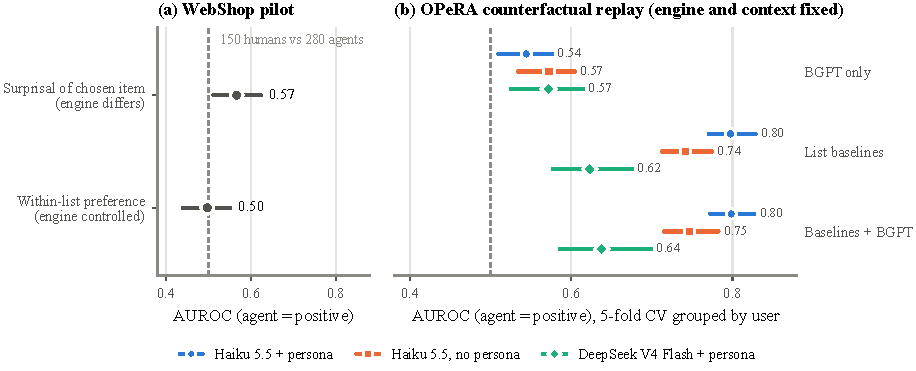
\includegraphics[width=\linewidth]{figures/fig_auroc.pdf}
\caption{\textbf{Detection performance with 95\% user-cluster bootstrap intervals.} (a) In the WebShop pilot, the apparent signal (agents less surprising) disappears once choices are scored within the list each chooser saw. (b) In counterfactual replay, \bgpt{} alone detects agents only weakly. Five list features detect them far better, and adding \bgpt{} to them changes AUROC by at most 0.015.}
\label{fig:auroc}
\end{figure}

\paragraph{Agents are too normal.} With engine and context fixed, all three agent conditions choose items that \bgpt{} ranks higher than the human's choice (Fig.~\ref{fig:shift}; Table~\ref{tab:main}). The mean within-list percentile rises from 0.59 to 0.64--0.67. The effect is significant in every condition (paired Wilcoxon $p=0.014$, $3.3\times10^{-5}$ and $2.6\times10^{-4}$) and holds for the conditional logit. This is the opposite of the assumption behind anomaly scoring: an agent operating inside an account makes the account look \emph{more} typical, not less, so a CUSUM on excess surprisal would drift away from an alarm.

\begin{figure}[t]
\centering
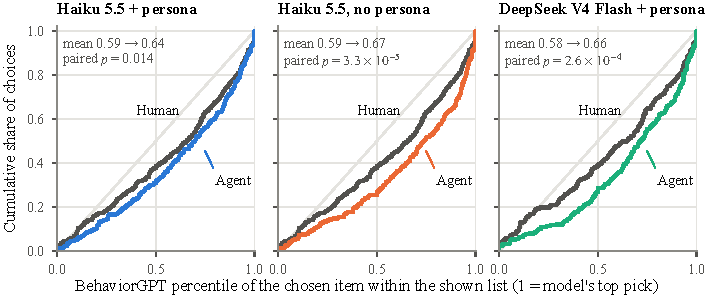
\includegraphics[width=\linewidth]{figures/fig_shift.pdf}
\caption{\textbf{Agents pick what the model expects.} Cumulative distribution of the \bgpt{} within-list percentile of the chosen item. Curves further to the right mean more model-typical choices. Human and agent choices are paired by step; $p$ from a paired Wilcoxon test.}
\label{fig:shift}
\end{figure}

\begin{table}[t]
\centering
\small
\caption{\textbf{\bgpt{} statistics, human vs.\ agent on identical context.} Means, paired Wilcoxon $p$, and AUROC at the step level (user-cluster bootstrap CI) and at the user level (per-user means, 45 vs.\ 45).}
\label{tab:main}
\setlength{\tabcolsep}{3.5pt}
\begin{tabular}{llcccc}
\toprule
Agent & Statistic & Human / Agent & Paired $p$ & Step AUROC & User AUROC \\
\midrule
Haiku 5.5 + persona & percentile & 0.590 / 0.635 & 0.014 & 0.54 [0.51, 0.58] & 0.61 \\
 & logit & 0.068 / 0.111 & 0.032 & 0.54 [0.50, 0.57] & 0.59 \\
 & history gain & 0.021 / 0.043 & 0.012 & 0.55 [0.51, 0.59] & 0.58 \\
\addlinespace
Haiku 5.5, no pers.\ & percentile & 0.590 / 0.670 & $3.3\times10^{-5}$ & 0.58 [0.54, 0.61] & 0.65 \\
 & logit & 0.068 / 0.156 & $1.5\times10^{-4}$ & 0.57 [0.54, 0.61] & 0.64 \\
 & history gain & 0.021 / 0.048 & 0.004 & 0.54 [0.50, 0.59] & 0.59 \\
\addlinespace
DeepSeek V4 Flash & percentile & 0.578 / 0.665 & $2.6\times10^{-4}$ & 0.58 [0.52, 0.63] & 0.62 \\
 & logit & 0.048 / 0.151 & $8.1\times10^{-4}$ & 0.57 [0.53, 0.63] & 0.61 \\
 & history gain & 0.001 / 0.029 & 0.019 & 0.55 [0.50, 0.59] & 0.58 \\
\bottomrule
\end{tabular}
\end{table}

\paragraph{But the signal is weak and redundant.} On its own, \bgpt{} reaches a step AUROC of 0.54--0.58, and 0.61--0.65 when averaged per user (Fig.~\ref{fig:auroc}b). The five list features alone reach 0.80 (Haiku with persona), 0.74 (Haiku without persona) and 0.62 (DeepSeek). Adding \bgpt{} changes these by $+0.001$, $+0.005$ and $+0.015$, all well inside the confidence intervals. The ROC curves for baselines and baselines + \bgpt{} overlap almost everywhere (Fig.~\ref{fig:roc}).

\paragraph{What gives agents away.} The cheap tells are behavioral, not semantic (Fig.~\ref{fig:tells}). Humans click a sponsored result in 34\% of steps, against 5\% for Haiku with persona and 23\% for DeepSeek. Haiku also reads deeper into the list (mean rank 18 vs.\ 8). All agents pick items with higher star ratings and more literal query matches. The last tell partly explains the \bgpt{} effect: given a query, the model favors on-topic, popular items, and so do agents.

\begin{figure}[t]
\centering
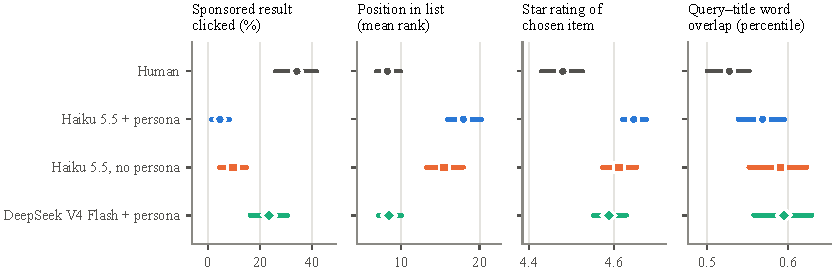
\includegraphics[width=\linewidth]{figures/fig_tells.pdf}
\caption{\textbf{Cheap tells.} Properties of the chosen item for humans and agents on the same 384 steps (247 for DeepSeek). Means with 95\% user-cluster bootstrap intervals. Agents avoid ads, prefer highly rated and literally matching items, and Haiku scrolls further down the list.}
\label{fig:tells}
\end{figure}

\paragraph{History and persona.} Conditioning on the user's history raises the percentile of human choices only from 0.569 to 0.590. In other words, the user's past actions add little predictive power for which listed item a person opens. For agents, history helps \emph{more} (history gain 0.03--0.05 vs.\ 0.00--0.02), probably because agents see the recent events in their prompt and stay consistent with them. Giving the agent the user's persona does not make it harder for \bgpt{} to detect (step AUROC 0.54 vs.\ 0.58 without persona; the intervals overlap). It does change its style: without the persona Haiku clicks more ads and stays higher in the list, which lowers the baseline detector from 0.80 to 0.74. The model family matters more than the persona: DeepSeek is the hardest agent to detect by any method.

\begin{figure}[t]
\centering
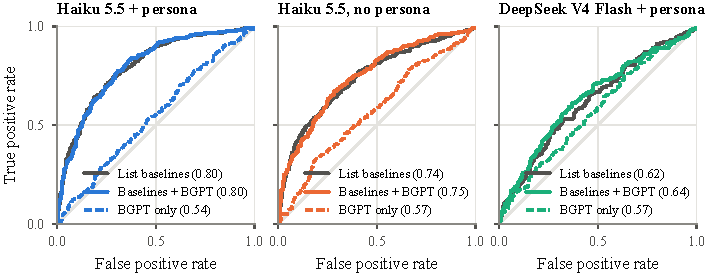
\includegraphics[width=\linewidth]{figures/fig_roc.pdf}
\caption{\textbf{ROC curves} for the three detectors (5-fold CV grouped by user; AUROC in parentheses). Adding \bgpt{} to the list baselines (solid colored line) barely moves the baseline curve (gray).}
\label{fig:roc}
\end{figure}
